% coding:utf-8

%----------------------------------------
%FOSAEBV, a LaTeX-Code for a summary of realtime image processing
%Copyright (C) 2013, Mario Felder

%This program is free software; you can redistribute it and/or
%modify it under the terms of the GNU General Public License
%as published by the Free Software Foundation; either version 2
%of the License, or (at your option) any later version.

%This program is distributed in the hope that it will be useful,
%but WITHOUT ANY WARRANTY; without even the implied warranty of
%MERCHANTABILITY or FITNESS FOR A PARTICULAR PURPOSE.  See the
%GNU General Public License for more details.
%----------------------------------------

\section{nichtlineare Filter}
\subsection{Rangordnungsoperatoren - Median-Filter}
Bei Randordnungsverfahren wird der Pixelwert anhand der Nachbarpixel neu gesetzt. Die grösse der Umgebung kann dabei variieren.
Bekannte Verfahren sind:
\begin{itemize}
	\item Minimum Filter: Es wird der minimale Pixelwert der Nachbarpixel gewählt
	\item Median Filter: Es wird der mittlere Pixelwert der Nachbarpixel gewählt
	\item Maximum Filter: Es wird der maximale Pixelwert der Nachbarpixel gewählt
\end{itemize}
~\\\\
Lösung in MATLAB:
\lstset{language=Matlab}
\lstinputlisting[firstline=1,caption=]{../Matlab/MedianFilter.m}
~\\

\subsection{morphologische Operatoren}
Bei morphologischen Operationen wird die Umgebung eines Pixels auf eine bestimmte Struktur hin untersucht.
Dazu wird ein Strukturelement verwendet, welches einen definierten Referenzpunkt hat.
\begin{center}
	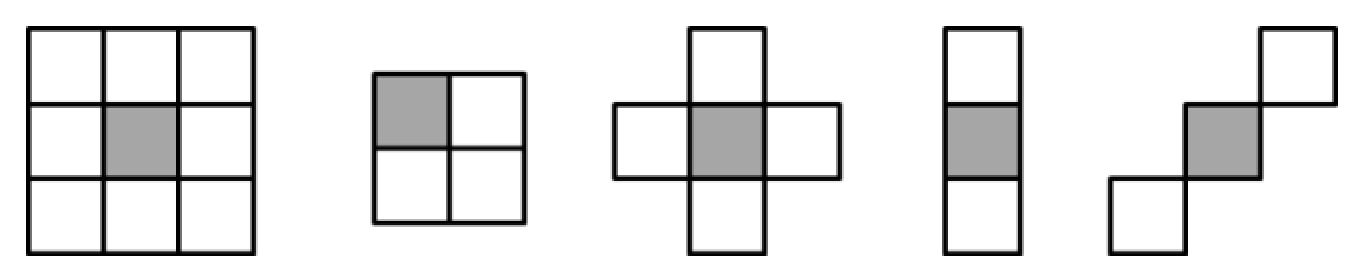
\includegraphics[scale=0.5]{../fig/structelem.png}
\end{center}
Morphologische Operatoren dienen dazu die Form von Objekten in definierte Weise zu verändern. 
Dies sind typisch:
\begin{itemize}
	\item Löschen kleiner Objekte (z.B. Pixelrauschen) 
	\item Schliessen von Löchern in Objekten
	\item Zusammenfassen von räumlich nahen Objekten
	\item Löschen aller Pixel im Inneren eines Objektes
	\item Reduzieren eines Objektes auf das Skelett
\end{itemize}

\subsubsection{Dilatation}
Bei der Dilatation wird das Strukturelement über das Bild geschoben.
Dabei werden alle Referenzpunkte des Strukturelementes markiert, bei denen eine nicht verschwindende Schnittmenge mit dem Objekt auftritt.
\begin{center}
	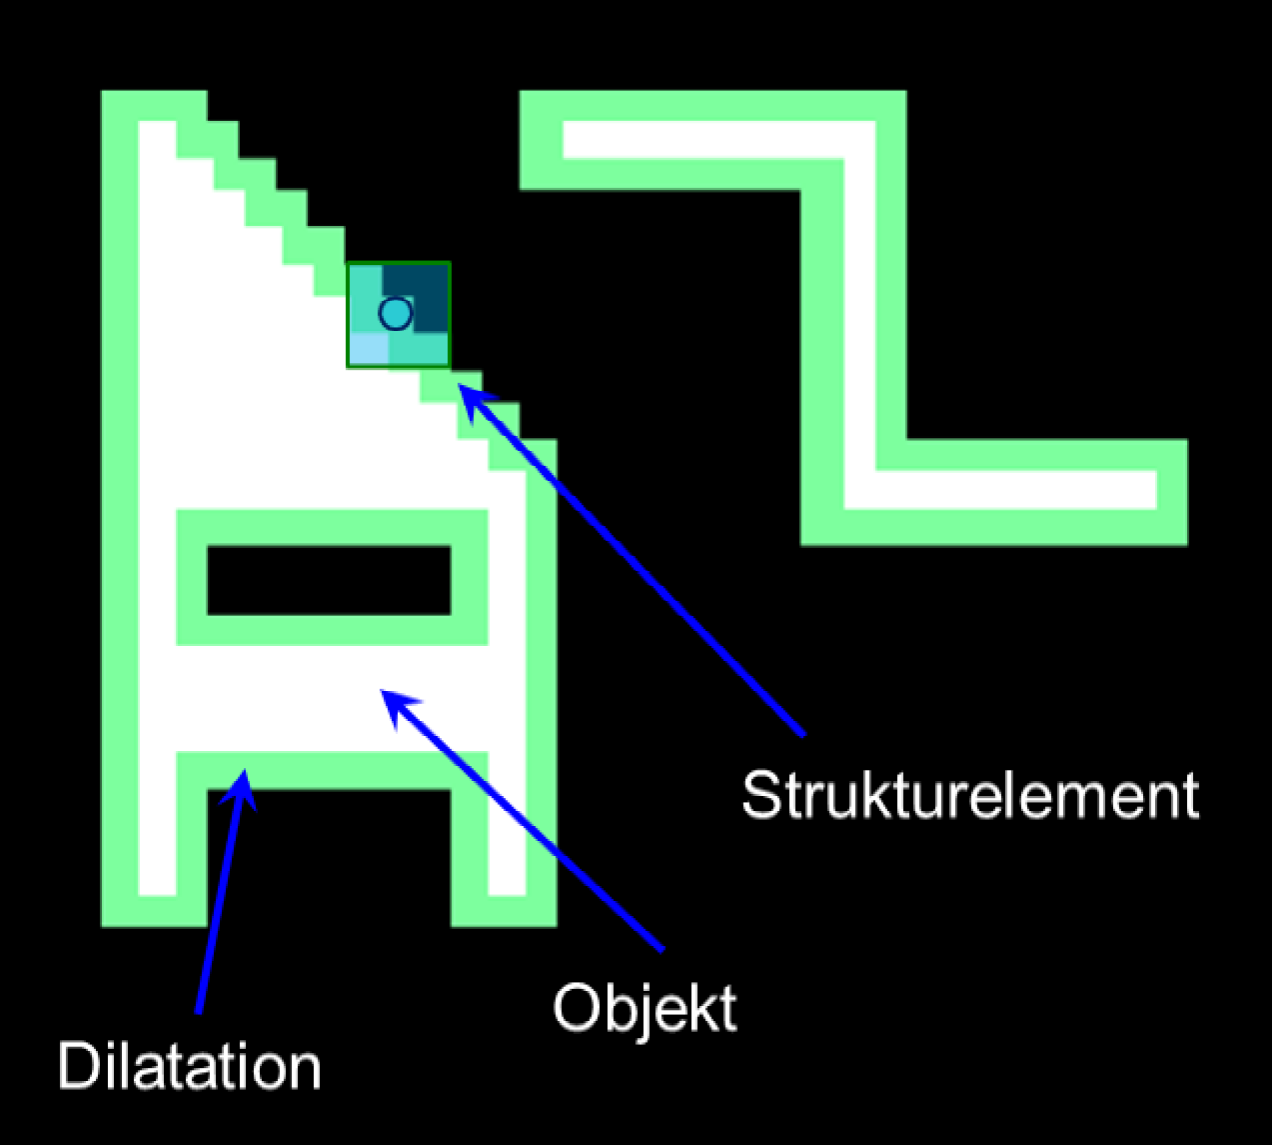
\includegraphics[scale=0.5]{../fig/dilatation.png}
\end{center}
Mathematische Beschreibung:
\[
	I \otimes h = \left\lbrace (m,n) | (\hat{h})_{m,n} \cap I \neq \{\} \right\rbrace
\]

\subsubsection{Erosion}
Bei der Dilatation wird das Strukturelement über das Bild geschoben.
Dabei werden alle Referenzpunkte des Strukturelementes markiert, bei denen das Strukturelement ganz in dem Objekt enthalten ist.
\begin{center}
	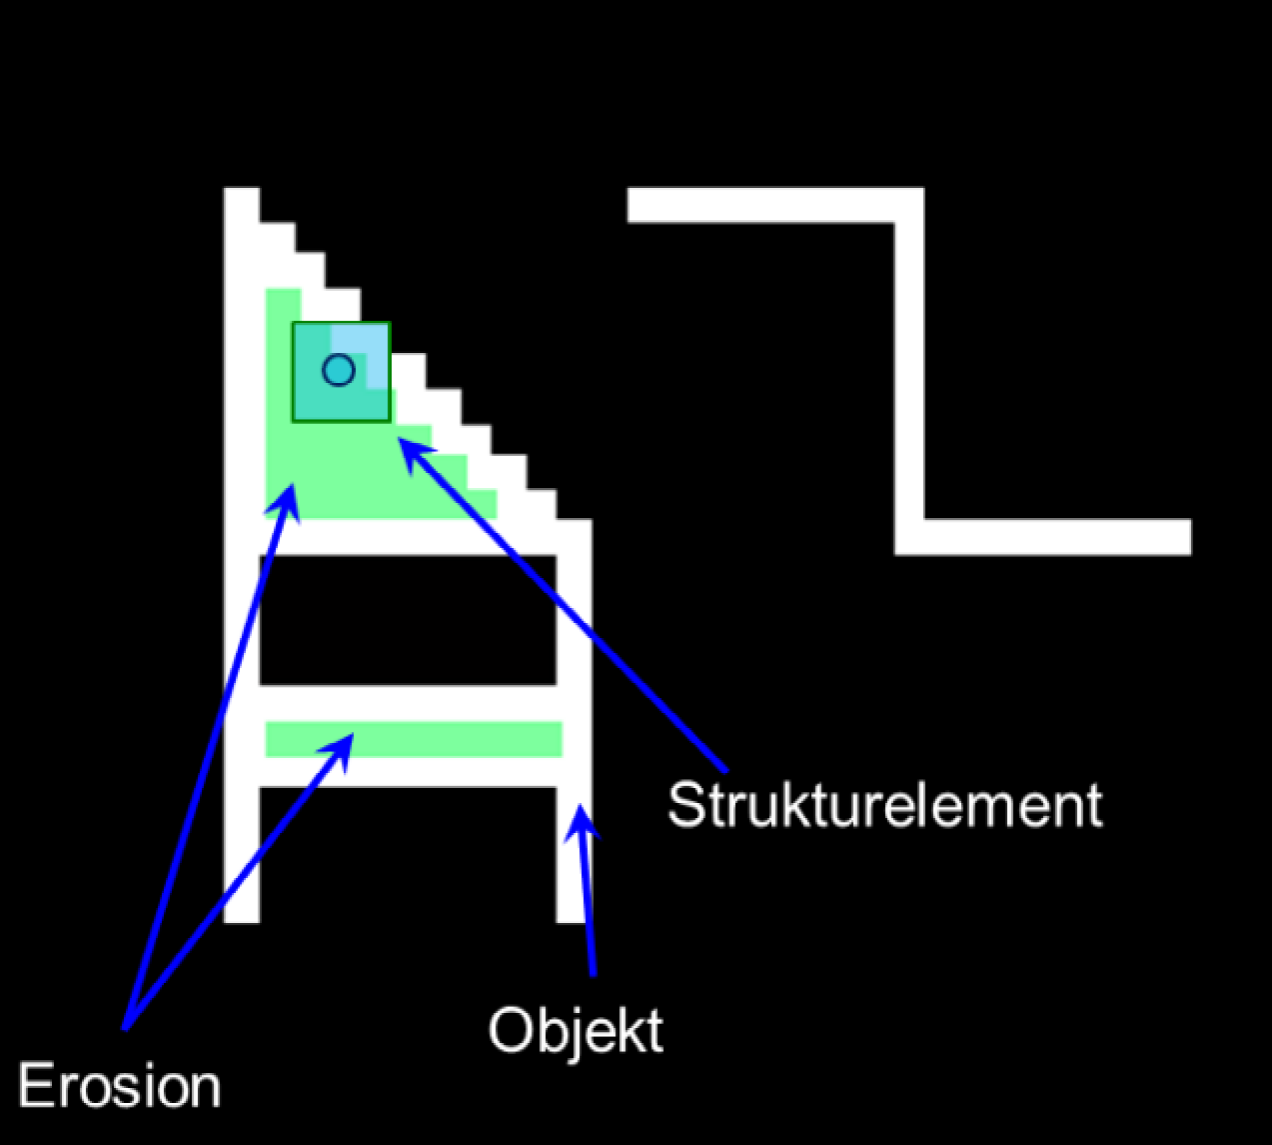
\includegraphics[scale=0.5]{../fig/erosion.png}
\end{center}
Mathematische Beschreibung:
\[
	I - h = \left\lbrace (m,n) | (h)_{m,n} \subset I \right\rbrace
\]

\subsubsection{Schliessung \& Öffnung}
Wen die Dilatation und Erosion kombiniert werden, entstehen weitere wichtige Operatoren.
Wird zuerst eine Dilatation dann eine Erosion ausgeführt, so entsteht eine Schliessung.
Umgekehrt eine Öffnung.
Mit der Schliessung können kleine Lücken geschlossen werden.
Die Öffnung kann Bildrauschen entfernen, da kleine Teile entfernt werden.\\
\\
Schliessung:
\[
	I \bullet h = (I \otimes h) - h
\]
~\\
Öffnung:
\[
	I \circ h = (I - h) \otimes h
\]
~\\\\
Lösung in MATLAB:
\lstset{language=Matlab}
\lstinputlisting[firstline=1,caption=]{../Matlab/morphologie.m}
~\\

\subsubsection{Hit- und Miss-Operation}
Bei dieser Operation wird nicht nur geschaut, ob das Strukturelement in einem Objekt enthalten ist, sondern ob die Nachbarschaft eine vorgegebene Struktur hat.
\begin{center}
	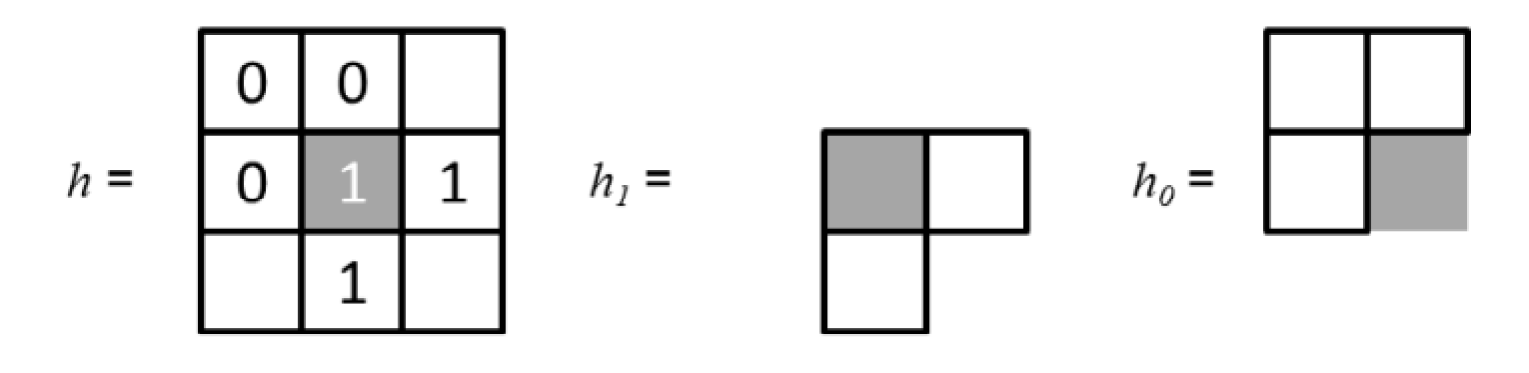
\includegraphics[scale=0.5]{../fig/hitmiss.png}
\end{center}
\begin{footnotesize}
	$0$: Das Pixel muss den Wert 0 haben\\
	$1$: Das Pixel muss den Wert 255 (bzw. 1) haben\\
	,,'': Der Wert des Pixels wird nicht in Betracht gezogen.\\
\end{footnotesize}
\\
Die mathematische Beschreibung:
\[
	I \pm h = (I - h_1) \cap (I^C - h_0)
\]
\begin{footnotesize}
	$I^C$: Das Komplement aller Pixel ungleich Null vom Bild $I$\\
\end{footnotesize}
\\
Hit- und Miss-Operation wird meist in Verbindung mit Verdünnungs- und Verdickungs-Operationen verwendet:
\[
	\text{thin}(I,h) = I \cap (I \pm h)^C
\]
